
\section{Resultados}
\label{sec:resultados}

Este capítulo presenta los resultados siguiendo el orden de las preguntas de
investigación: primero qué casos resultaron combinables y por qué se
descartaron los demás (RQ1); después con qué intensidad bajó la complejidad
cognitiva en los casos elegibles (RQ2), con su validación de contraste frente
a SonarQube; y por último cómo se comportaron los modelos de lenguaje sobre el
mismo problema (RQ3). Todas las cifras de complejidad proceden del proxy del
prototipo (\autoref{sec:proxy}) y de los artefactos generados; los estadísticos descriptivos se han calculado sobre esos
mismos ficheros y ninguno se ha estimado a mano para esta memoria.

\subsection{RQ1 — Taxonomía de aplicabilidad}
\label{sec:resultados-rq1}
Sobre el corpus consolidado de 126 casos (8 piloto y 118 reales), el detector
marcó como elegibles 104 y descartó 22. La cifra interesa menos por sí misma
que por su lectura: en un corpus dominado por código real de proyectos
abiertos, una mayoría amplia de los patrones \lstinline|if|--\lstinline|if|
examinados sí admite la combinación bajo P1--P5.

Más revelador es el reparto de los motivos de descarte, que es justamente lo
que da respuesta empírica a RQ1: \emph{\textquestiondown{}en qué casos no se
pueden combinar?} La \autoref{tab:descartes} y la \autoref{fig:descartes}
reproducen la frecuencia de cada categoría tal como la emite el pipeline.
Conviene leerlas con una advertencia: los motivos se agregan por candidato y
un mismo método puede aportar varios, de modo que la suma supera el número de
casos inelegibles; no es un error, sino el modo en que
\lstinline|detectWithReasons| reporta la evidencia.

\begin{table}[ht]
\centering
\caption{Frecuencia de motivos de descarte en el corpus consolidado.
Fuente: \texttt{output/rq2-batch/rq2-summary.md}.}
\label{tab:descartes}
\begin{tabular}{@{}lr@{}}
\toprule
\textbf{Categoría (\texttt{DiscardReason})} & \textbf{Apariciones} \\
\midrule
\texttt{SINGLE\_STATEMENT\_NOT\_IF}            & 16 \\
\texttt{METHOD\_CALL\_IN\_CONDITION} (P5)      & 5 \\
\texttt{OUTER\_BLOCK\_MULTIPLE\_STATEMENTS} (P2) & 5 \\
(sin patrón de \lstinline|if| anidado)         & 5 \\
\texttt{OUTER\_HAS\_ELSE} (P1)                 & 4 \\
\texttt{INNER\_HAS\_ELSE} (P4)                 & 1 \\
\texttt{ASSIGNMENT\_IN\_CONDITION} (P5)        & 1 \\
\texttt{INCREMENT\_OR\_DECREMENT\_IN\_CONDITION} (P5) & 1 \\
\bottomrule
\end{tabular}
\end{table}

\begin{figure}[ht]
\centering
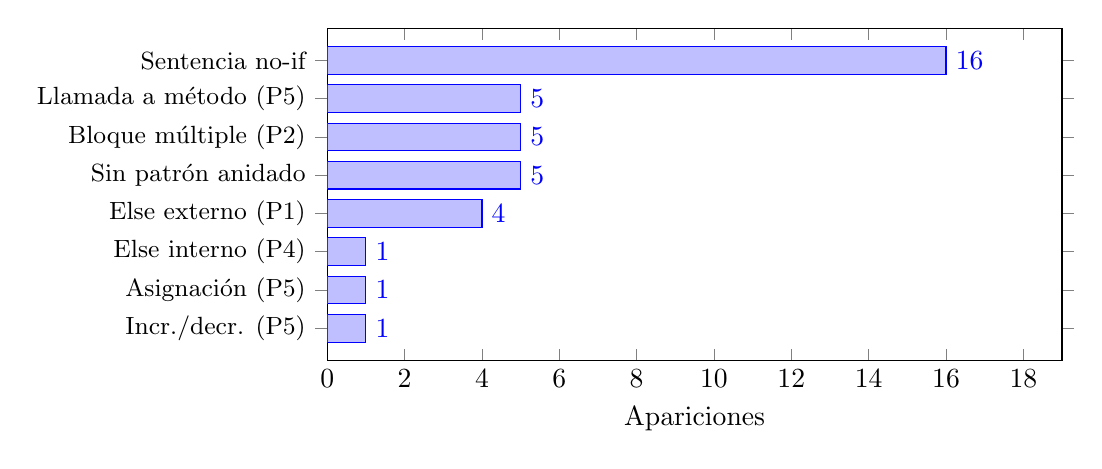
\begin{tikzpicture}
\begin{axis}[
  width=0.9\linewidth, height=5.8cm,
  xbar, xmin=0, xmax=19,
  xlabel={Apariciones},
  symbolic y coords={{Incr./decr. (P5)},{Asignación (P5)},{Else interno (P4)},{Else externo (P1)},{Sin patrón anidado},{Bloque múltiple (P2)},{Llamada a método (P5)},{Sentencia no-if}},
  ytick=data, nodes near coords, nodes near coords align={horizontal},
  enlarge y limits=0.12, y tick label style={font=\small},
]
\addplot+[fill=blue!25] coordinates {
  (1,{Incr./decr. (P5)}) (1,{Asignación (P5)}) (1,{Else interno (P4)})
  (4,{Else externo (P1)}) (5,{Sin patrón anidado}) (5,{Bloque múltiple (P2)})
  (5,{Llamada a método (P5)}) (16,{Sentencia no-if}) };
\end{axis}
\end{tikzpicture}
\caption{Distribución de los motivos de descarte (RQ1). Fuente:
\texttt{output/rq2-batch/rq2-summary.md}.}
\label{fig:descartes}
\end{figure}

De aquí se extraen dos lecturas. La primera es que el grueso de los descartes
no se debe a que la combinación sea insegura, sino a que el patrón objetivo
simplemente no está presente: la sentencia única del bloque externo no es un
\lstinline|if| anidado (\texttt{SINGLE\_STATEMENT\_NOT\_IF}, el motivo más
frecuente, con 16 apariciones). La segunda es que, cuando el patrón sí aparece
pero se rechaza, el bloqueo proviene sobre todo de P5 —y dentro de P5, de las
llamadas a método en la condición—, seguido de los bloques externos con más de
una sentencia. En otras palabras, en código real el principal enemigo de la
combinación segura no es el \lstinline|else|, sino el posible efecto colateral
escondido en la condición. Este resultado respalda, a posteriori, la decisión
de diseño de tratar P5 de forma sintáctica y conservadora.

\subsection{RQ2 — Impacto en la complejidad cognitiva}
\label{sec:resultados-rq2}
La respuesta cuantitativa a RQ2 es directa: sobre los 104 casos elegibles, la
complejidad cognitiva agregada (proxy) se reduce en $\Delta = -278$, lo que
supone una reducción relativa del 9{,}8\,\% sobre la complejidad total de esos
métodos (de 2825 a 2547 puntos). La reducción no se concentra en unos pocos
casos: los 104 elegibles presentan, sin excepción, un $\Delta$ negativo
(media $-2{,}67$ puntos por caso, desviación típica $2{,}29$). Los 22 casos
inelegibles mantienen, por construcción, $\Delta = 0$.

La \autoref{tab:rq2-cinco} resume la distribución completa mediante los
estadísticos descriptivos de la complejidad antes y después de refactorizar y
de su diferencia. La \autoref{fig:boxplots} los representa como diagramas de
caja y la \autoref{fig:hist-delta} muestra el histograma de las reducciones.

\begin{table}[ht]
\centering
\caption{Estadísticos descriptivos sobre los 104 casos elegibles (CC proxy):
mínimo, cuartiles, mediana, máximo, media y desviación típica. Cuartiles por
interpolación lineal. Fuente: \texttt{output/rq2-batch/rq2-all-results.csv}.}
\label{tab:rq2-cinco}
\begin{tabular}{@{}lrrrrrrrr@{}}
\toprule
\textbf{Métrica} & \textbf{n} & \textbf{mín} & \textbf{Q1} & \textbf{mediana} & \textbf{Q3} & \textbf{máx} & \textbf{media} & \textbf{sd} \\
\midrule
CC antes   & 104 & 3   & 4    & 10{,}5 & 20{,}25 & 228 & 27{,}16 & 46{,}01 \\
CC después & 104 & 2   & 3    & 8      & 18{,}25 & 220 & 24{,}49 & 44{,}44 \\
$\Delta$   & 104 & $-14$ & $-3$ & $-2$ & $-1$    & $-1$ & $-2{,}67$ & 2{,}29 \\
\bottomrule
\end{tabular}
\end{table}

El rango intercuartílico pasa de $16{,}25$ (antes) a $15{,}25$ (después): la
caja de la complejidad se desplaza hacia abajo tras refactorizar (la mediana
baja de $10{,}5$ a $8$ y el tercer cuartil de $20{,}25$ a $18{,}25$), con una
cola larga de métodos muy complejos —hasta 228, varios de Knowage— que
aparecen como valores atípicos según el criterio de Tukey. El histograma de
$\Delta$ confirma la asimetría del efecto: el 50\,\% central de las reducciones
se sitúa entre $-1$ y $-3$ (mediana $-2$), y la gran mayoría de los casos
ahorran uno o dos puntos, con una cola de reducciones mayores que llega a
$-14$.

\begin{figure}[ht]
\centering
\begin{tikzpicture}
\begin{axis}[
  width=0.52\linewidth, height=6cm,
  ymode=log, ymin=1, ymax=320,
  ylabel={Complejidad cognitiva (proxy, log)},
  xtick={1,2}, xticklabels={Antes, Después},
  boxplot/draw direction=y, log ticks with fixed point,
]
\addplot+[boxplot prepared={lower whisker=3, lower quartile=4, median=10.5, upper quartile=20.25, upper whisker=42}]
  coordinates {(0,46)(0,52)(0,53)(0,57)(0,63)(0,63)(0,157)(0,165)(0,166)(0,166)(0,167)(0,183)(0,183)(0,228)};
\addplot+[boxplot prepared={lower whisker=2, lower quartile=3, median=8, upper quartile=18.25, upper whisker=39}]
  coordinates {(0,44)(0,48)(0,52)(0,57)(0,58)(0,150)(0,158)(0,159)(0,159)(0,160)(0,176)(0,176)(0,220)};
\end{axis}
\end{tikzpicture}\hfill
\begin{tikzpicture}
\begin{axis}[
  width=0.40\linewidth, height=6cm,
  ylabel={$\Delta$ CC (proxy)}, xtick={1}, xticklabels={$\Delta$},
  boxplot/draw direction=y,
]
\addplot+[boxplot prepared={lower whisker=-6, lower quartile=-3, median=-2, upper quartile=-1, upper whisker=-1}]
  coordinates {(0,-14)(0,-9)(0,-8)(0,-8)(0,-8)(0,-7)(0,-7)(0,-7)(0,-7)(0,-7)(0,-7)(0,-7)};
\end{axis}
\end{tikzpicture}
\caption{Diagramas de caja (104 casos elegibles, CC proxy). Izquierda:
complejidad antes vs.\ después (escala logarítmica; los puntos son valores
atípicos según el criterio de Tukey de $1{,}5\cdot\mathrm{IQR}$). Derecha:
distribución de la reducción $\Delta$. Datos: \texttt{output/rq2-batch/}.}
\label{fig:boxplots}
\end{figure}

\begin{figure}[ht]
\centering
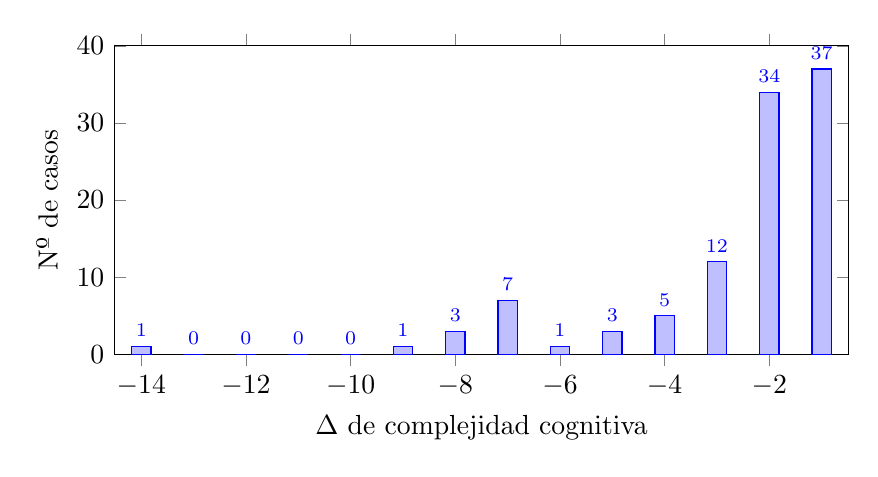
\begin{tikzpicture}
\begin{axis}[
  ybar, width=0.9\linewidth, height=5.5cm,
  xlabel={$\Delta$ de complejidad cognitiva}, ylabel={Nº de casos},
  xtick={-14,-12,-10,-8,-6,-4,-2}, ymin=0, ymax=40, bar width=7pt,
  nodes near coords, every node near coord/.append style={font=\scriptsize},
  enlarge x limits=0.04,
]
\addplot+[fill=blue!25] coordinates {
  (-14,1)(-13,0)(-12,0)(-11,0)(-10,0)(-9,1)(-8,3)(-7,7)(-6,1)(-5,3)(-4,5)(-3,12)(-2,34)(-1,37)};
\end{axis}
\end{tikzpicture}
\caption{Histograma de la reducción $\Delta$ sobre los 104 casos elegibles
(CC proxy). La masa se concentra en reducciones pequeñas ($-1$, $-2$), con una
cola de reducciones mayores. Datos: \texttt{output/rq2-batch/rq2-all-results.csv}.}
\label{fig:hist-delta}
\end{figure}

Más allá de la distribución, el detalle por caso
(\autoref{tab:rq2-destacados}) muestra dos comportamientos complementarios. En
métodos pequeños, combinar un único anidamiento ahorra uno o dos puntos. En
métodos grandes y muy anidados —habituales en el corpus real— el ahorro
absoluto crece, aunque sigue acotado por el hecho de que cada aplicación
elimina un solo nivel de anidamiento. El caso de mayor reducción individual es
\texttt{CYBERCAPTOR\_VERTEX\_GET\_RELATED\_MACHINE}, que baja de 52 a 38
($\Delta=-14$).

\begin{table}[ht]
\centering
\caption{Casos destacados de RQ2 (proxy). El conjunto completo de los 126
casos está en \texttt{output/rq2-batch/rq2-summary.md} y en el Apéndice~E.}
\label{tab:rq2-destacados}
\begin{tabular}{@{}lrrrr@{}}
\toprule
\textbf{caseId} & \textbf{Aplic.} & \textbf{CC antes} & \textbf{CC después} & \textbf{$\Delta$} \\
\midrule
\texttt{CYBERCAPTOR\_VERTEX\_GET\_RELATED\_MACHINE} & 1 & 52 & 38 & $-14$ \\
\texttt{ANT\_STRIP\_JAVA\_COMMENTS\_READ}           & 1 & 57 & 48 & $-9$ \\
\texttt{KNOWAGE\_DOCUMENT\_EXECUTION\_RESOURCE\_GET\dots} & 1 & 228 & 220 & $-8$ \\
\texttt{JACKSON\_CORE\dots SKIP\_COLON\_FAST}       & 2 & 36 & 28 & $-8$ \\
\texttt{REAL\_COMMONS\_LANG\_CONTAINS\_NONE}        & 1 & 15 & 11 & $-4$ \\
\texttt{PILOT\_VALID\_NESTED\_IN\_LOOP}             & 1 & 6  & 4  & $-2$ \\
\texttt{PILOT\_VALID\_SIMPLE}                       & 1 & 3  & 2  & $-1$ \\
\texttt{REAL\_COMMONS\_MATH\_VALIDATE\_RANGE} (P1)  & 0 & 4  & 4  & $0$ \\
\bottomrule
\end{tabular}
\end{table}

De esta observación se desprende un matiz honesto que conviene no maquillar: la
transformación mejora la legibilidad local, pero no \emph{arregla} un método
intrínsecamente complejo. Un método con complejidad 228 sigue siendo difícil
después de bajar a 220. El valor de la refactorización está en eliminar
anidamiento accidental allí donde lo hay, no en rescatar diseños que arrastran
problemas más profundos.

\subsection{Eliminación de issues de SonarQube}
\label{sec:resultados-issues}
La reducción de complejidad tiene una consecuencia práctica que va más allá del
$\Delta$. SonarQube marca un \emph{issue} de mantenibilidad cuando la
complejidad cognitiva de un método supera el umbral por defecto de 15 de su
regla S3776. Tiene sentido, por tanto, preguntarse en cuántos casos la
refactorización hace \emph{desaparecer} ese issue, es decir, cuántos métodos
cruzan de $\text{CC}>15$ a $\text{CC}\le 15$ (\autoref{tab:issues-sonar}).

\begin{table}[ht]
\centering
\caption{Cruce del umbral de issue de SonarQube ($\text{CC}=15$) en los 104
casos elegibles (CC proxy). Fuente: \texttt{output/rq2-batch/rq2-all-results.csv}.}
\label{tab:issues-sonar}
\begin{tabular}{@{}lr@{}}
\toprule
\textbf{Situación} & \textbf{Casos} \\
\midrule
Con issue antes ($\text{CC}>15$)                 & 41 \\
\quad $\rightarrow$ issue \textbf{eliminado} ($\text{CC}\le 15$ después) & 6 \\
\quad $\rightarrow$ issue persiste ($\text{CC}>15$ después)             & 35 \\
Sin issue ya antes ($\text{CC}\le 15$)           & 63 \\
\bottomrule
\end{tabular}
\end{table}

De los 104 casos elegibles, 41 superaban el umbral antes de refactorizar. Tras
aplicar la transformación, 6 de ellos bajan a 15 o menos —el issue desaparece
sin tocar la semántica— y 35 siguen por encima. Los 63 restantes ya estaban en
zona sin issue. Dicho de otro modo, la refactorización elimina el issue de
SonarQube en el 14{,}6\,\% de los métodos que lo tenían. La lectura honesta de
este dato encaja con la de RQ2: la combinación elimina el issue sobre todo
cuando el método estaba \emph{cerca} del umbral; en los métodos muy complejos
(los de Knowage, con CC entre 150 y 228) reduce la complejidad pero una sola
combinación no basta para cruzar el umbral. El efecto, por tanto, es local y
acotado, pero tangible: seis issues de mantenibilidad menos a coste cero en
términos de comportamiento.

\subsection{Validación de contraste con SonarQube}
\label{sec:resultados-sonar}
La métrica de RQ2 es un proxy, y por eso se contrasta con la implementación
oficial de SonarQube sobre un subset de cuatro casos (\autoref{sec:sonar-val}).
El artefacto \texttt{output/rq2-sonar-validation/rq2-sonar-validation.md}
recoge una coincidencia exacta entre proxy y SonarQube en las ocho medidas del
subset (cuatro \emph{before} y cuatro \emph{after}), con $\Sigma\Delta = -8$ en
ambos.

\pendienteverif{} \textbf{Este resultado no se da por confirmado.} Los
artefactos del repositorio son contradictorios: mientras la tabla anterior y la
cabecera del documento declaran una ejecución real completada, el fichero
\texttt{metadata.json} anota expresamente que \emph{«no se han ejecutado
escaneos reales de SonarQube en esta entrega»}, y la sección de trazabilidad
del propio informe deja la versión exacta, las fechas y el \emph{commit hash}
marcados como pendientes. Hasta que se ejecute la corrida real y se completen
esos campos con valores independientes del proxy, esta validación se presenta
como \textbf{provisional}. La incertidumbre afecta solo a este contraste; los
resultados de RQ2 (\autoref{sec:resultados-rq2}) se sostienen sobre el proxy y
son independientes de él.

\subsection{RQ3 — Refactorización por modelos de lenguaje}
\label{sec:resultados-rq3}
La campaña real (fase~9, modo \emph{live}) ejecutó las 300 invocaciones
previstas —50 casos $\times$ 2 modelos $\times$ 3 intentos— sin ningún
incidente técnico. El subconjunto de 50 casos (36 elegibles y 14 no elegibles)
amplía sustancialmente la evaluación respecto a versiones anteriores del
protocolo y permite analizar el comportamiento de los modelos no solo de forma
agregada, sino separando los casos que \emph{deben} transformarse de los que
\emph{deben} rechazarse. La \autoref{tab:rq3-modelo} y la
\autoref{fig:rq3-verdictos} resumen el desempeño por modelo.

\begin{table}[ht]
\centering
\caption{Resultados de RQ3 por modelo (150 invocaciones por modelo). Tasa de
éxito = veredictos \texttt{SUCCESS}; coincidencia con \emph{baseline} =
salida idéntica al baseline determinista; consistencia = pares caso--modelo
cuyos tres intentos coinciden. Fuente:
\texttt{output/rq3-campaign-limited/rq3-aggregated.md}.}
\label{tab:rq3-modelo}
\begin{tabular}{@{}lrrrrrr@{}}
\toprule
\textbf{Modelo} & \textbf{ÉXITO} & \textbf{INCORR.} & \textbf{ABSTEN.} & \textbf{Tasa éxito} & \textbf{Coinc.\ baseline} & \textbf{Consist.} \\
\midrule
\texttt{gpt-4o}  & 122 & 0 & 28 & 81{,}3\,\% & 78{,}7\,\% & 96{,}0\,\% \\
\texttt{gpt-4.1} & 145 & 5 & 0  & 96{,}7\,\% & 94{,}0\,\% & 98{,}0\,\% \\
\bottomrule
\end{tabular}
\end{table}

\begin{figure}[ht]
\centering
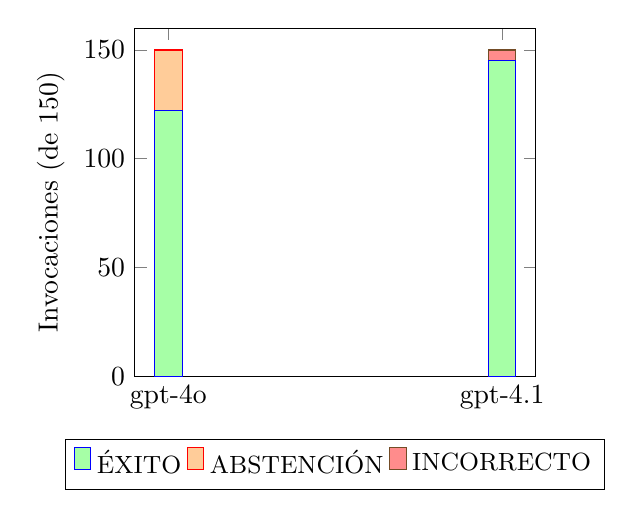
\begin{tikzpicture}
\begin{axis}[
  ybar stacked, width=0.55\linewidth, height=6cm,
  symbolic x coords={gpt-4o,gpt-4.1}, xtick=data,
  ylabel={Invocaciones (de 150)}, ymin=0, ymax=160,
  legend style={at={(0.5,-0.18)}, anchor=north, legend columns=3, font=\small},
]
\addplot+[fill=green!35] coordinates {(gpt-4o,122)(gpt-4.1,145)};
\addplot+[fill=orange!40] coordinates {(gpt-4o,28)(gpt-4.1,0)};
\addplot+[fill=red!45]   coordinates {(gpt-4o,0)(gpt-4.1,5)};
\legend{ÉXITO, ABSTENCIÓN, INCORRECTO}
\end{axis}
\end{tikzpicture}\hfill
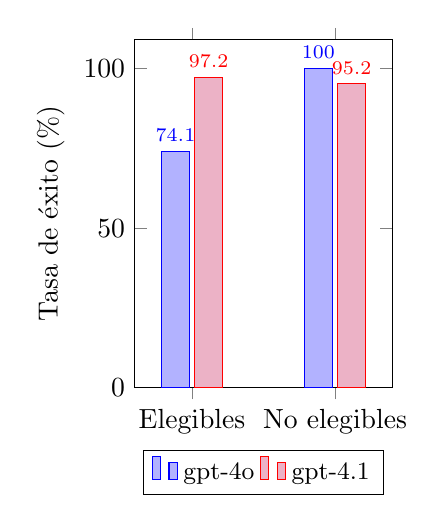
\begin{tikzpicture}
\begin{axis}[
  ybar, width=0.40\linewidth, height=6cm,
  symbolic x coords={Elegibles,No elegibles}, xtick=data,
  ylabel={Tasa de éxito (\%)}, ymin=0, ymax=109,
  nodes near coords, every node near coord/.append style={font=\scriptsize},
  legend style={at={(0.5,-0.18)}, anchor=north, legend columns=2, font=\small},
  enlarge x limits=0.4,
]
\addplot+[fill=blue!30]  coordinates {(Elegibles,74.1)(No elegibles,100)};
\addplot+[fill=purple!30] coordinates {(Elegibles,97.2)(No elegibles,95.2)};
\legend{gpt-4o, gpt-4.1}
\end{axis}
\end{tikzpicture}
\caption{RQ3 (300 invocaciones). Izquierda: reparto de veredictos por modelo.
Derecha: tasa de éxito separando casos elegibles (deben transformarse) de no
elegibles (deben rechazarse). Datos:
\texttt{output/rq3-campaign-limited/rq3-summary.csv}.}
\label{fig:rq3-verdictos}
\end{figure}

La fotografía agregada esconde lo más interesante, que aparece al separar los
casos por elegibilidad (\autoref{tab:rq3-elegibilidad}). Los dos modelos
exhiben perfiles opuestos ante la decisión de \emph{si transformar}:

\begin{table}[ht]
\centering
\caption{Tasa de éxito de RQ3 por categoría de elegibilidad (intentos
agregados; 36 casos elegibles $\times 3$ y 14 no elegibles $\times 3$ por
modelo). Fuente: \texttt{output/rq3-campaign-limited/rq3-summary.csv}.}
\label{tab:rq3-elegibilidad}
\begin{tabular}{@{}lrr@{}}
\toprule
\textbf{Modelo} & \textbf{Elegibles ($n=108$)} & \textbf{No elegibles ($n=42$)} \\
\midrule
\texttt{gpt-4o}  & 80/108 \;(74{,}1\,\%)  & 42/42 \;(100{,}0\,\%) \\
\texttt{gpt-4.1} & 105/108 \;(97{,}2\,\%) & 40/42 \;(95{,}2\,\%) \\
\bottomrule
\end{tabular}
\end{table}

\texttt{gpt-4o} es \textbf{conservador}: no produce ni una sola transformación
incorrecta (0 \texttt{INCORRECT}) y rechaza correctamente los 42 intentos sobre
casos no elegibles (100\,\%); pero esa cautela tiene un coste, porque se
abstiene también en casos que sí debían transformarse, y su acierto sobre los
elegibles cae al 74{,}1\,\%. Sus 28 abstenciones recaen, todas, sobre casos
elegibles. \texttt{gpt-4.1} muestra el perfil \textbf{opuesto}: aplica la
transformación con acierto en el 97{,}2\,\% de los elegibles, pero a cambio se
equivoca en 5 ocasiones (las únicas \texttt{INCORRECT} de toda la campaña),
algunas de ellas transformando casos que debían rechazarse (95{,}2\,\% en no
elegibles). En términos clásicos, \texttt{gpt-4o} prioriza la precisión a costa
de la cobertura y \texttt{gpt-4.1} la cobertura a costa de algún falso
positivo. El \emph{baseline} determinista, por construcción, no incurre en
ninguno de los dos errores.

La consistencia a temperatura cero es alta en ambos modelos (96{,}0\,\% y
98{,}0\,\% de los pares caso--modelo con los tres intentos idénticos), lo que
indica que los aciertos y los fallos descritos son criterios estables de cada
modelo y no ruido de muestreo. En cuanto al coste de invocación, el tiempo de
respuesta por llamada tuvo una mediana de 1066\,ms y una media de 1649\,ms, en
un rango de 436 a 9350\,ms. Un caso resulta especialmente ilustrativo:
\texttt{ANT\_U\_R\_L\_RESOURCE\_GET\_U\_R\_L}, elegible, en el que \emph{ambos}
modelos fallaron en los tres intentos —\texttt{gpt-4o} por abstención y
\texttt{gpt-4.1} por transformación incorrecta—, lo que muestra que la
dificultad no siempre está en la elegibilidad nominal del caso. El detalle
caso por caso se conserva en
\texttt{output/rq3-campaign-limited/rq3-summary.csv}.

\subsection{Validación humana del pipeline automático}
\label{sec:validacion-humana}
El pipeline se ha construido con asistencia intensiva de herramientas de IA y,
además, sus etapas son automáticas: la detección de \lstinline|if| anidados, la
comprobación de las precondiciones P1--P5 y el cálculo de la complejidad
cognitiva. Para acotar la confianza en esos resultados se incorpora una
\textbf{validación humana} sobre una muestra aleatoria, con un principio
sencillo: tomar $N$ casos al azar, comprobar manualmente si el veredicto
automático es correcto y reportar el porcentaje de acierto por etapa.

\paragraph{Protocolo.} Se extrae una muestra de 30 casos del corpus
consolidado —20 elegibles y 10 no elegibles— mediante muestreo aleatorio
reproducible (semilla fija 42). Para cada caso, un revisor humano abre el
fichero fuente y el resultado automático y emite un veredicto
(correcto/incorrecto) en cuatro etapas: (i)~detección del patrón de
\lstinline|if| anidado; (ii)~cumplimiento o incumplimiento de las
precondiciones y su motivo de descarte; (iii)~complejidad cognitiva
\emph{before}; y (iv)~complejidad cognitiva \emph{after}. El instrumento de
recogida está en \texttt{output/rq2-human-validation/validation-sample.csv} y
el procedimiento completo en \texttt{docs/human-validation-protocol.md}.

\paragraph{Resultados.} \pendienteverif{} Pendiente de completar la inspección
manual. La \autoref{tab:validacion-humana} recoge la plantilla; el porcentaje
de acierto por etapa, con su intervalo de confianza de Wilson al 95\,\%, se
rellenará al cerrar la revisión.

\begin{table}[ht]
\centering
\caption{Validación humana del pipeline (muestra $N=30$, semilla 42).
Plantilla a completar tras la inspección manual.}
\label{tab:validacion-humana}
\begin{tabular}{@{}lccc@{}}
\toprule
\textbf{Etapa} & \textbf{Aciertos/$N$} & \textbf{\% acierto} & \textbf{IC 95\,\% (Wilson)} \\
\midrule
Detección de \lstinline|if| anidados      & --- & --- & --- \\
Precondiciones P1--P5 (y motivo)          & --- & --- & --- \\
Complejidad cognitiva \emph{before}       & --- & --- & --- \\
Complejidad cognitiva \emph{after}        & --- & --- & --- \\
\bottomrule
\end{tabular}
\end{table}

\subsection{Discusión integrada}
Leídos en conjunto, los tres resultados se refuerzan. RQ1 acota dónde la
combinación es segura y muestra que el principal obstáculo en código real es el
posible efecto colateral en la condición, no el \lstinline|else|. RQ2 confirma
que, donde es segura, la combinación reduce de forma sistemática la complejidad
cognitiva —los 104 casos elegibles mejoran—, con un efecto modesto pero
consistente y un puñado de issues de SonarQube eliminados. Y RQ3, ya sobre 50
casos, aporta el matiz más fino para responder a
\emph{«\textquestiondown{}pueden los LLM hacerlo de forma correcta y
automática?»}: los modelos saben aplicar la transformación cuando procede, pero
difieren en la frontera difícil, que no es transformar, sino \emph{abstenerse}
cuando una precondición lo prohíbe. Un modelo peca de conservador y otro de
confiado, y solo el \emph{baseline} determinista acierta en ambos extremos por
construcción. Es ahí donde el prototipo aporta su mayor valor: como referencia
fiable frente a la que medir, precisamente, esa frontera.
